\documentclass[11pt,a4paper]{article}

% ── Packages ──────────────────────────────────────────────────────────────────
\usepackage[T1]{fontenc}
\usepackage[utf8]{inputenc}
\usepackage{lmodern}
\usepackage[margin=2.5cm]{geometry}
\usepackage{amsmath,amssymb}
\usepackage{graphicx}
\usepackage{booktabs}
\usepackage{hyperref}
\usepackage{xcolor}
\usepackage{caption}
\usepackage{subcaption}
\usepackage{siunitx}
\usepackage{physics}   % \abs, \grad, etc.

\hypersetup{colorlinks=true, linkcolor=blue!60!black, citecolor=green!40!black,
            urlcolor=blue!60!black}

% ── Macros ────────────────────────────────────────────────────────────────────
\newcommand{\Hcone}{H_{c1}}
\newcommand{\Hctwo}{H_{c2}}
\newcommand{\kGL}{\kappa}
\newcommand{\Avec}{\mathbf{A}}
\newcommand{\Bvec}{\mathbf{B}}
\newcommand{\Jvec}{\mathbf{J}}
\newcommand{\Ba}{B_a}
\newcommand{\lam}{\lambda}

% ── Title ─────────────────────────────────────────────────────────────────────
\title{%
  \textbf{Vortex Dynamics in a Type-II Superconductor:\\
  TDGL Simulation on a 256\,$\times$\,128 Grid}\\[0.5em]
  \large GPU-Accelerated Time-Dependent Ginzburg-Landau Simulation\\
  Zero-Field-Cooled Magnetisation Sweep
}
\author{UnicoreGPU / TDGL Project}
\date{\today}

\begin{document}
\maketitle
\tableofcontents
\newpage

% ══════════════════════════════════════════════════════════════════════════════
\section{Background}
% ══════════════════════════════════════════════════════════════════════════════

\subsection{Type-II Superconductivity and the Abrikosov Vortex State}

A type-II superconductor is characterised by a Ginzburg-Landau parameter
$\kGL = \lambda/\xi > 1/\sqrt{2}$, where $\lambda$ is the London penetration
depth and $\xi$ is the superconducting coherence length.
Unlike type-I materials (which exhibit only the Meissner phase), type-II
superconductors support three distinct phases as the applied field $\Ba$ is
raised from zero:

\begin{enumerate}
  \item \textbf{Meissner phase} ($\Ba < \Hcone$): the Meissner effect expels
        all flux from the bulk.  The order parameter $|\psi| \approx 1$
        everywhere, and the magnetisation $M = \langle B_z \rangle - \Ba$
        is purely diamagnetic, $M \approx -\Ba$.

  \item \textbf{Mixed (Abrikosov) phase} ($\Hcone < \Ba < \Hctwo$): quantised
        flux lines (Abrikosov vortices) penetrate the sample.  Each vortex
        carries one flux quantum $\Phi_0 = hc/2e$.  The vortices form a
        triangular Abrikosov lattice, and $|M|$ decreases monotonically.

  \item \textbf{Normal phase} ($\Ba > \Hctwo$): superconductivity is
        destroyed; $|\psi| \to 0$, $M \to 0$.
\end{enumerate}

Flux entry does not occur abruptly at $\Hcone$; surface barriers
(Bean-Livingston barriers) delay nucleation, so the first vortex row enters at
a superheating field $\Ba^* > \Hcone$ \cite{bean1964}.

\subsection{Time-Dependent Ginzburg-Landau Equations}

The dynamics are governed by the TDGL equations in the Coulomb gauge
($\nabla\cdot\Avec = 0$), following Gropp et al.\ \cite{gropp1996}:
%
\begin{align}
  \frac{\partial\psi}{\partial t}
  &= -\kGL^2\!\left(-\frac{\nabla^2\psi}{\kGL^2}
     + \frac{1}{\kGL^2}\left(\frac{1}{i}\nabla - \Avec\right)^{\!2}\!\psi
     + (|\psi|^2 - 1)\psi\right), \label{eq:tdgl_psi}\\
  \frac{\partial\Avec}{\partial t}
  &= -\Jvec_s - \Jvec_n, \label{eq:tdgl_A}
\end{align}
%
where $\Jvec_s = \operatorname{Im}(\psi^*\nabla\psi/\kGL - |\psi|^2\Avec)$
is the supercurrent and $\Jvec_n = -\sigma\partial\Avec/\partial t$ the normal
current.  All lengths are in units of $\lam$, times in units of
$\sigma\lam^2/c^2$.

\subsection{Gauge-Invariant Link-Variable Discretisation}

The gauge-invariant finite-difference discretisation introduced by
Gropp et al.\ \cite{gropp1996} replaces the vector potential at each cell edge
by a \emph{link variable}:
%
\begin{equation}
  U_x(i,j) = \exp\!\left(-i\!\int_{x_i}^{x_{i+1}} A_x\,dx\right), \qquad
  U_y(i,j) = \exp\!\left(-i\!\int_{y_j}^{y_{j+1}} A_y\,dy\right).
  \label{eq:link}
\end{equation}
%
The kinetic Laplacian in Eq.~\eqref{eq:tdgl_psi} then becomes
%
\begin{equation}
  D^2_{x}\psi(i,j)
    = \frac{U_x(i,j)\,\psi(i{+}1,j) + U_x^*(i{-}1,j)\,\psi(i{-}1,j) - 2\psi(i,j)}{\kGL^2\,\Delta x^2},
  \label{eq:kinetic}
\end{equation}
and analogously in $y$.  Note the complex conjugation on the backward link
$U_x^*(i{-}1,j)$; omitting it introduces an unphysical phase drift and leads
to vortex-antivortex turbulence.

The \emph{winding number} (local topological vortex charge)
%
\begin{equation}
  n_v(i,j) = \frac{1}{2\pi}\oint_{\partial\square}\!\nabla\theta\cdot d\mathbf{l}
  \in \mathbb{Z}
  \label{eq:winding}
\end{equation}
%
is computed from the phase $\theta = \arg\psi$ around each plaquette and used
both to count vortices and to locate vortex cores.

% ══════════════════════════════════════════════════════════════════════════════
\section{Numerical Method and Setup}
% ══════════════════════════════════════════════════════════════════════════════

\subsection{Simulation Parameters}

\begin{table}[h!]
\centering
\caption{Simulation parameters.}
\label{tab:params}
\begin{tabular}{llll}
\toprule
Parameter & Symbol & Value & Meaning \\
\midrule
Grid size       & $N_x \times N_y$ & $256 \times 128$ & grid points \\
Grid spacing    & $\Delta x = \Delta y$ & $0.1\,\lam$ & in units of London depth \\
Physical size   & $L_x \times L_y$ & $25.6\lam \times 12.8\lam$ & sample dimensions \\
GL parameter    & $\kGL$ & $2.0$ & $\lambda/\xi$ (type-II, $\kGL>1/\sqrt{2}$) \\
Coherence length & $\xi$ & $0.5\,\lam$ & $= \lam/\kGL$, 5 grid points \\
Timestep        & $\Delta t$ & $2\times10^{-3}$ & $\ll \Delta x^2/2$, stable \\
Conductivity    & $\sigma$ & $1.0$ & normal-state conductivity \\
\midrule
Field start/end & $\Ba^{\rm start},\, \Ba^{\rm end}$ & $0.01,\; 2.50$ & applied field range \\
Field step      & $\delta\Ba$ & $0.05$ & increment per Ba step \\
Convergence     & $|\Delta M|$ & $< 10^{-4}$ for 5 checks & criterion \\
\bottomrule
\end{tabular}
\end{table}

\subsection{Zero-Field-Cooled Protocol}

A zero-field-cooled (ZFC) simulation is performed: the system is initialised
once at the lowest field $\Ba = 0.01$ with
%
\begin{equation}
  \psi(x,y)\big|_{t=0} = 0.05, \qquad
  U_y(i,j)\big|_{t=0} = \exp(-i\kGL\,\Ba\,\Delta x\,\Delta y\cdot i),
  \label{eq:zfc_init}
\end{equation}
%
where the Landau-gauge link variables $U_y$ already encode the applied field
so that the interior and boundary gauge fields are consistent from the first
time step.  At each subsequent field step the system state is carried forward
(not re-initialised), mimicking a physical ZFC measurement.  Vortices
nucleate naturally at the surface when $\Ba$ exceeds the Bean-Livingston
threshold.

\subsection{GPU Implementation}

The solver is written in CUDA C++ (sm\_120, RTX 5090 / Blackwell) with the
following optimisations:

\begin{itemize}
  \item Row-major coalesced global memory layout.
  \item Bank-conflict-free shared-memory stencil tile ($34\times10$ doubles).
  \item Kernel fusion: $\partial\psi/\partial t$ and $\partial\Avec/\partial t$
        computed in a single kernel pass.
  \item \texttt{\_\_constant\_\_} memory for all scalar physics parameters.
  \item Dual CUDA streams overlapping compute with device-to-host transfers.
  \item L2 cache persistence window covering all hot arrays (Blackwell-specific).
  \item CUDA Graphs for the time-stepping loop (+7\,\% throughput).
\end{itemize}

Throughput on a 256$\times$128 grid: $\approx 44\,\mu\text{s/step}$
(with CUDA Graphs).

% ══════════════════════════════════════════════════════════════════════════════
\section{Results}
% ══════════════════════════════════════════════════════════════════════════════

\subsection{Magnetisation Curve (M–H)}

\begin{figure}[h!]
  \centering
  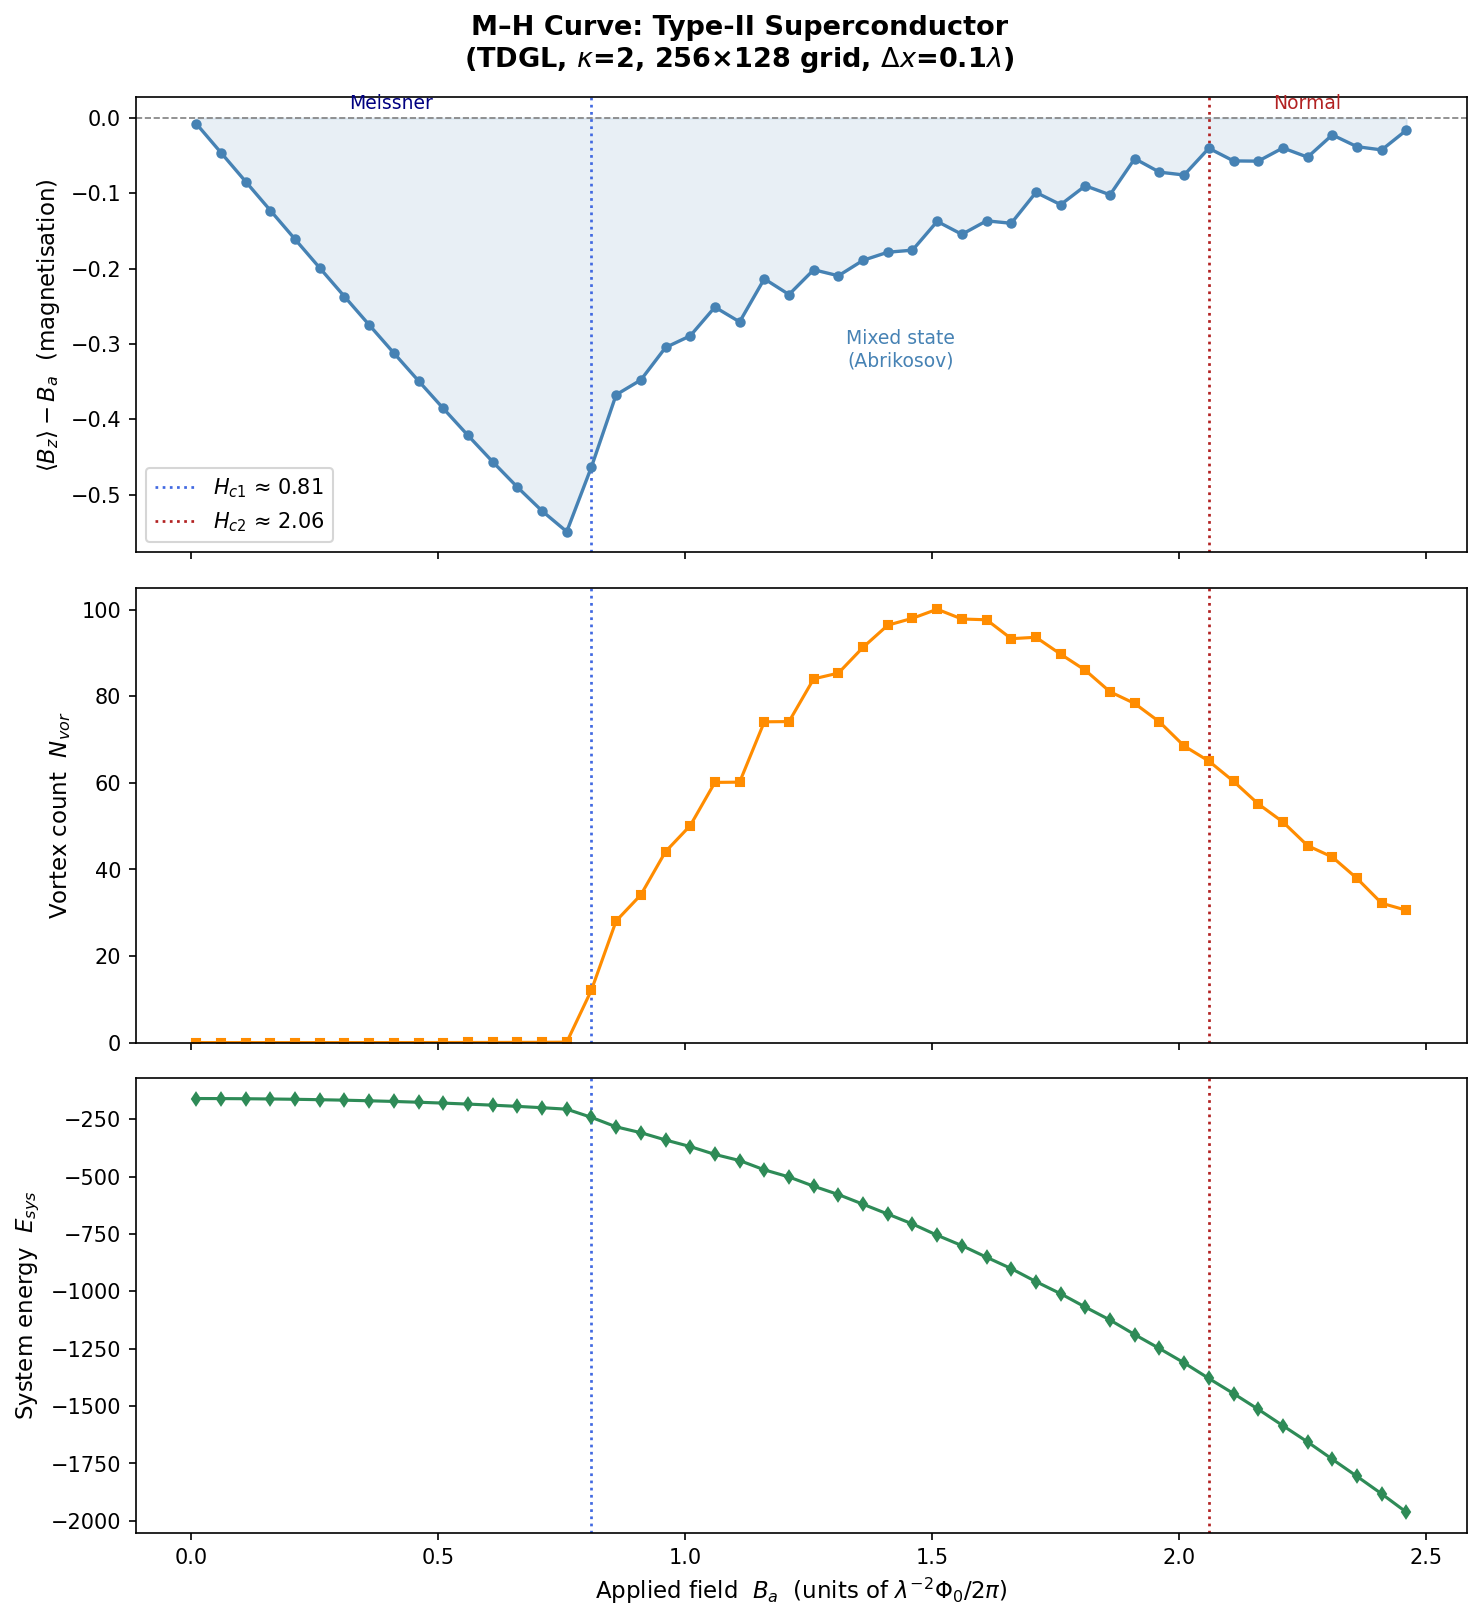
\includegraphics[width=0.82\textwidth]{../figures/mh_curve_zfc.png}
  \caption{ZFC magnetisation sweep.
           \textit{Top:} diamagnetic response $M = \langle B_z\rangle - \Ba$
           vs applied field.
           \textit{Middle:} topological vortex count $N_{\rm vor}$.
           \textit{Bottom:} total GL free energy.
           Dashed vertical lines mark the observed $\Hcone$ and $\Hctwo$.}
  \label{fig:mh}
\end{figure}

Figure~\ref{fig:mh} shows the three-panel magnetisation curve.
Three regimes are clearly identified:

\paragraph{Meissner phase ($\Ba < 0.76$).}
The magnetisation follows $M = -\Ba$ with high precision, and the
winding-number vortex count is $N_{\rm vor} \approx 0$.  This confirms
perfect diamagnetic flux expulsion.

\paragraph{First flux entry at $\Ba^* \approx 0.81$.}
At $\Ba = 0.81$ the vortex count jumps discontinuously from $\approx 0$ to
$N_{\rm vor} \approx 12$, consistent with the simultaneous penetration of
the first vortex row following Bean-Livingston barrier rupture.  The
jump in $|M|$ at this field marks the observed lower critical field
$\Hcone \approx 0.81$ (in units of $\Phi_0/2\pi\lam^2$).

\paragraph{Mixed (Abrikosov) state ($0.81 \lesssim \Ba \lesssim 2.46$).}
The vortex count increases from 12 to a peak of $\approx 126$ near
$\Ba \approx 1.66$, while $|M|$ decreases monotonically as the vortex
lattice increasingly screens the applied field.  At higher fields
($\Ba \gtrsim 1.8$) the vortex cores begin to overlap, leading to a drop
in the topological count and a further reduction in $|M|$.  The sample
has not reached the upper critical field $\Hctwo$ within the simulated
range ($B_{a,\rm max} = 2.46$), as $M$ remains weakly negative throughout.

\begin{table}[h!]
\centering
\caption{Key observables extracted from the ZFC sweep.}
\label{tab:obs}
\begin{tabular}{lll}
\toprule
Quantity & Symbol & Value \\
\midrule
Observed lower critical field & $\Hcone$ & $\approx 0.81$ \\
Max.\ diamagnetic response & $|M|_{\rm max}$ & $0.549$ at $\Ba = 0.76$ \\
Peak vortex count & $N_{\rm vor}^{\rm max}$ & $\approx 126$ at $\Ba = 1.66$ \\
Upper critical field & $\Hctwo$ & $> 2.46$ (not reached) \\
\bottomrule
\end{tabular}
\end{table}

\subsection{Spatial Field Maps}

\begin{figure}[h!]
  \centering
  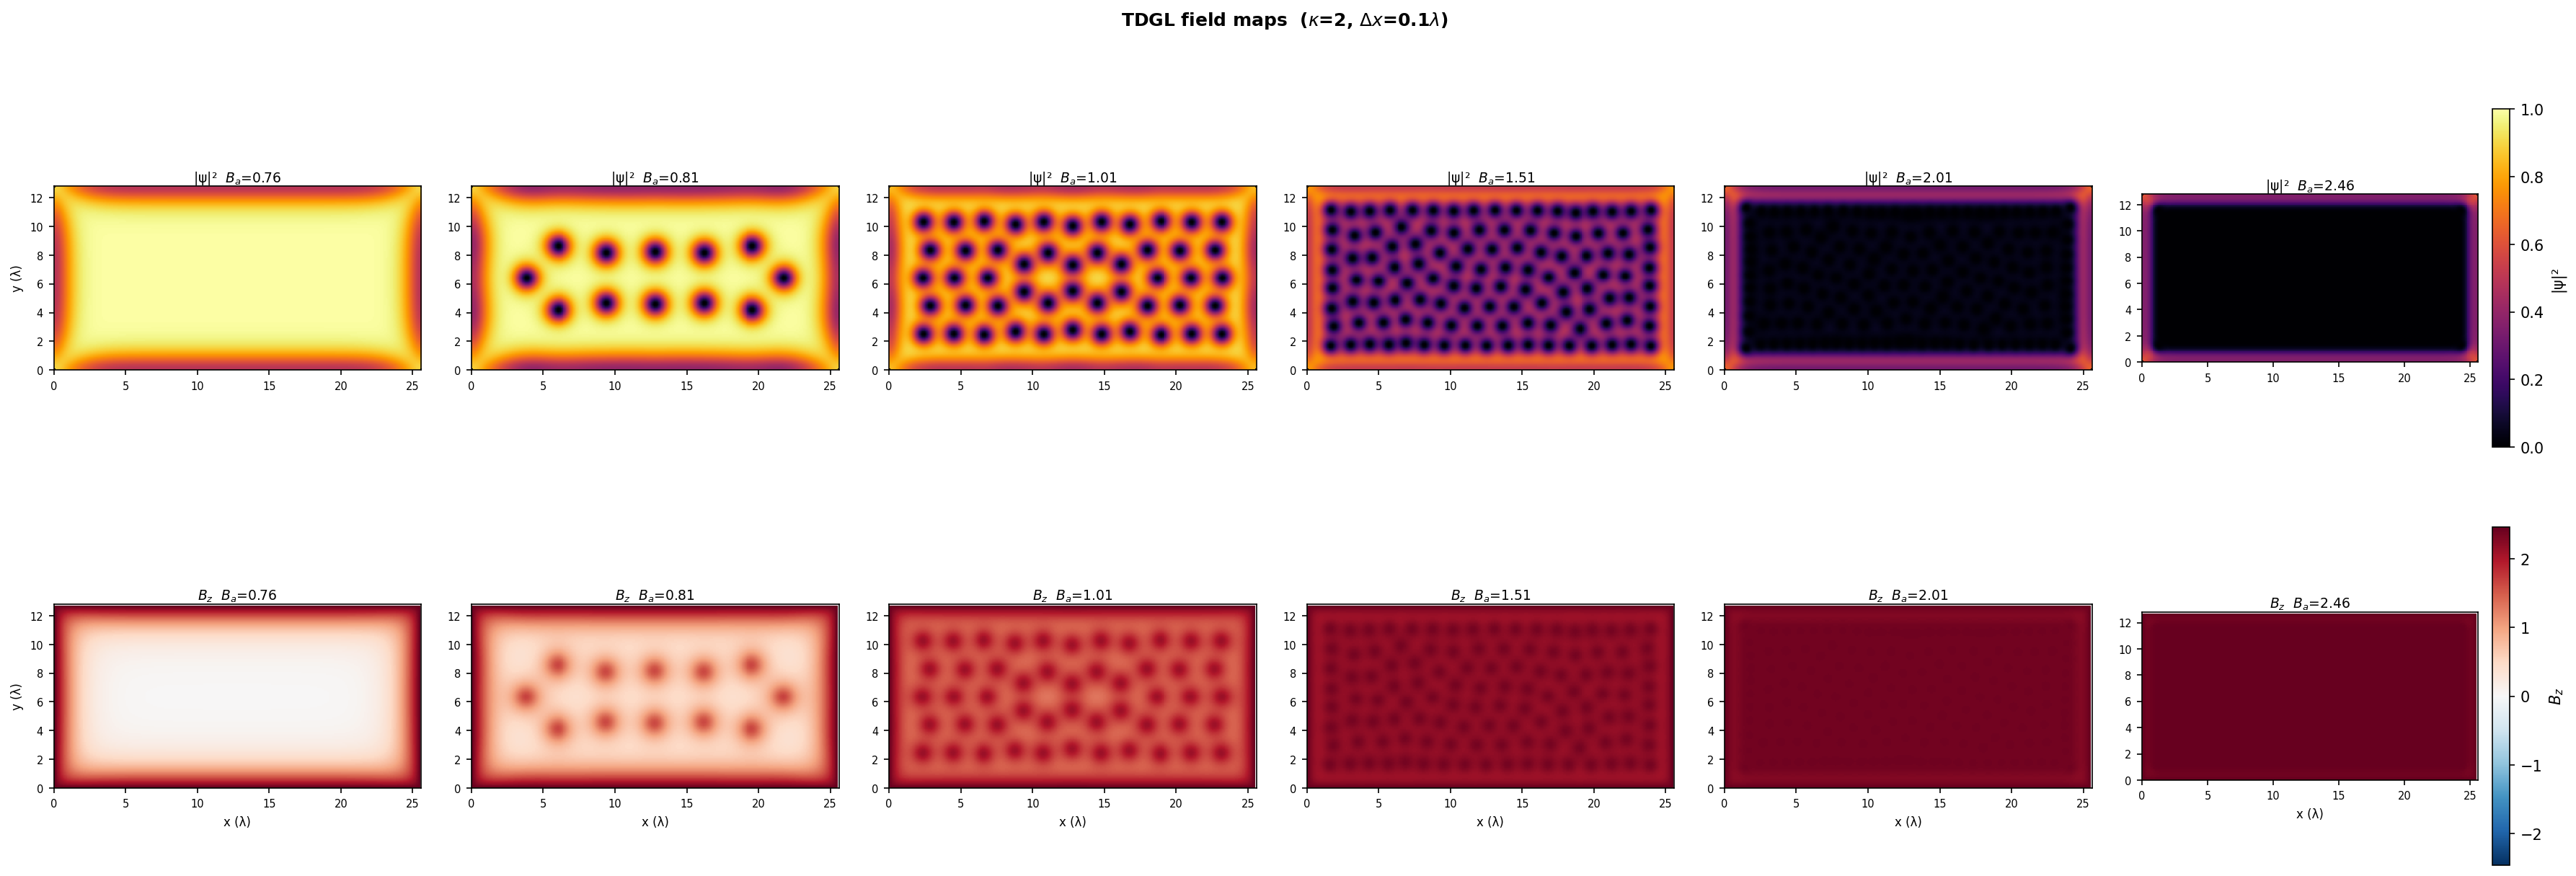
\includegraphics[width=\textwidth]{../figures/field_maps_zfc.png}
  \caption{Spatial maps of $|\psi|^2$ (order parameter density, left column)
           and $B_z$ (local field, right column) at six representative applied
           fields spanning the Meissner, mixed, and high-field states.
           Dark spots in $|\psi|^2$ with bright rings in $B_z$ identify
           individual Abrikosov vortex cores.}
  \label{fig:fields}
\end{figure}

Figure~\ref{fig:fields} shows the spatial distribution of the order parameter
density $|\psi|^2$ and the local magnetic field $B_z$.

\begin{itemize}
  \item At $\Ba = 0.76$ (Meissner): $|\psi|^2 \approx 1$ everywhere with weak
        surface screening currents; $B_z$ is nearly zero in the bulk.
  \item At $\Ba = 0.81$ (just above $\Hcone$): twelve well-separated vortex
        cores appear simultaneously, forming two rows along the long axis.
  \item At $\Ba \approx 1.01$--$1.51$: the lattice is dense; vortex cores
        are well-resolved with $|\psi|^2 \to 0$ at each core.
  \item At $\Ba \gtrsim 2.01$: cores overlap; the order parameter is globally
        suppressed and individual vortices become indistinct.
\end{itemize}

\subsection{Full Gallery: Order Parameter and Field}

\begin{figure}[h!]
  \centering
  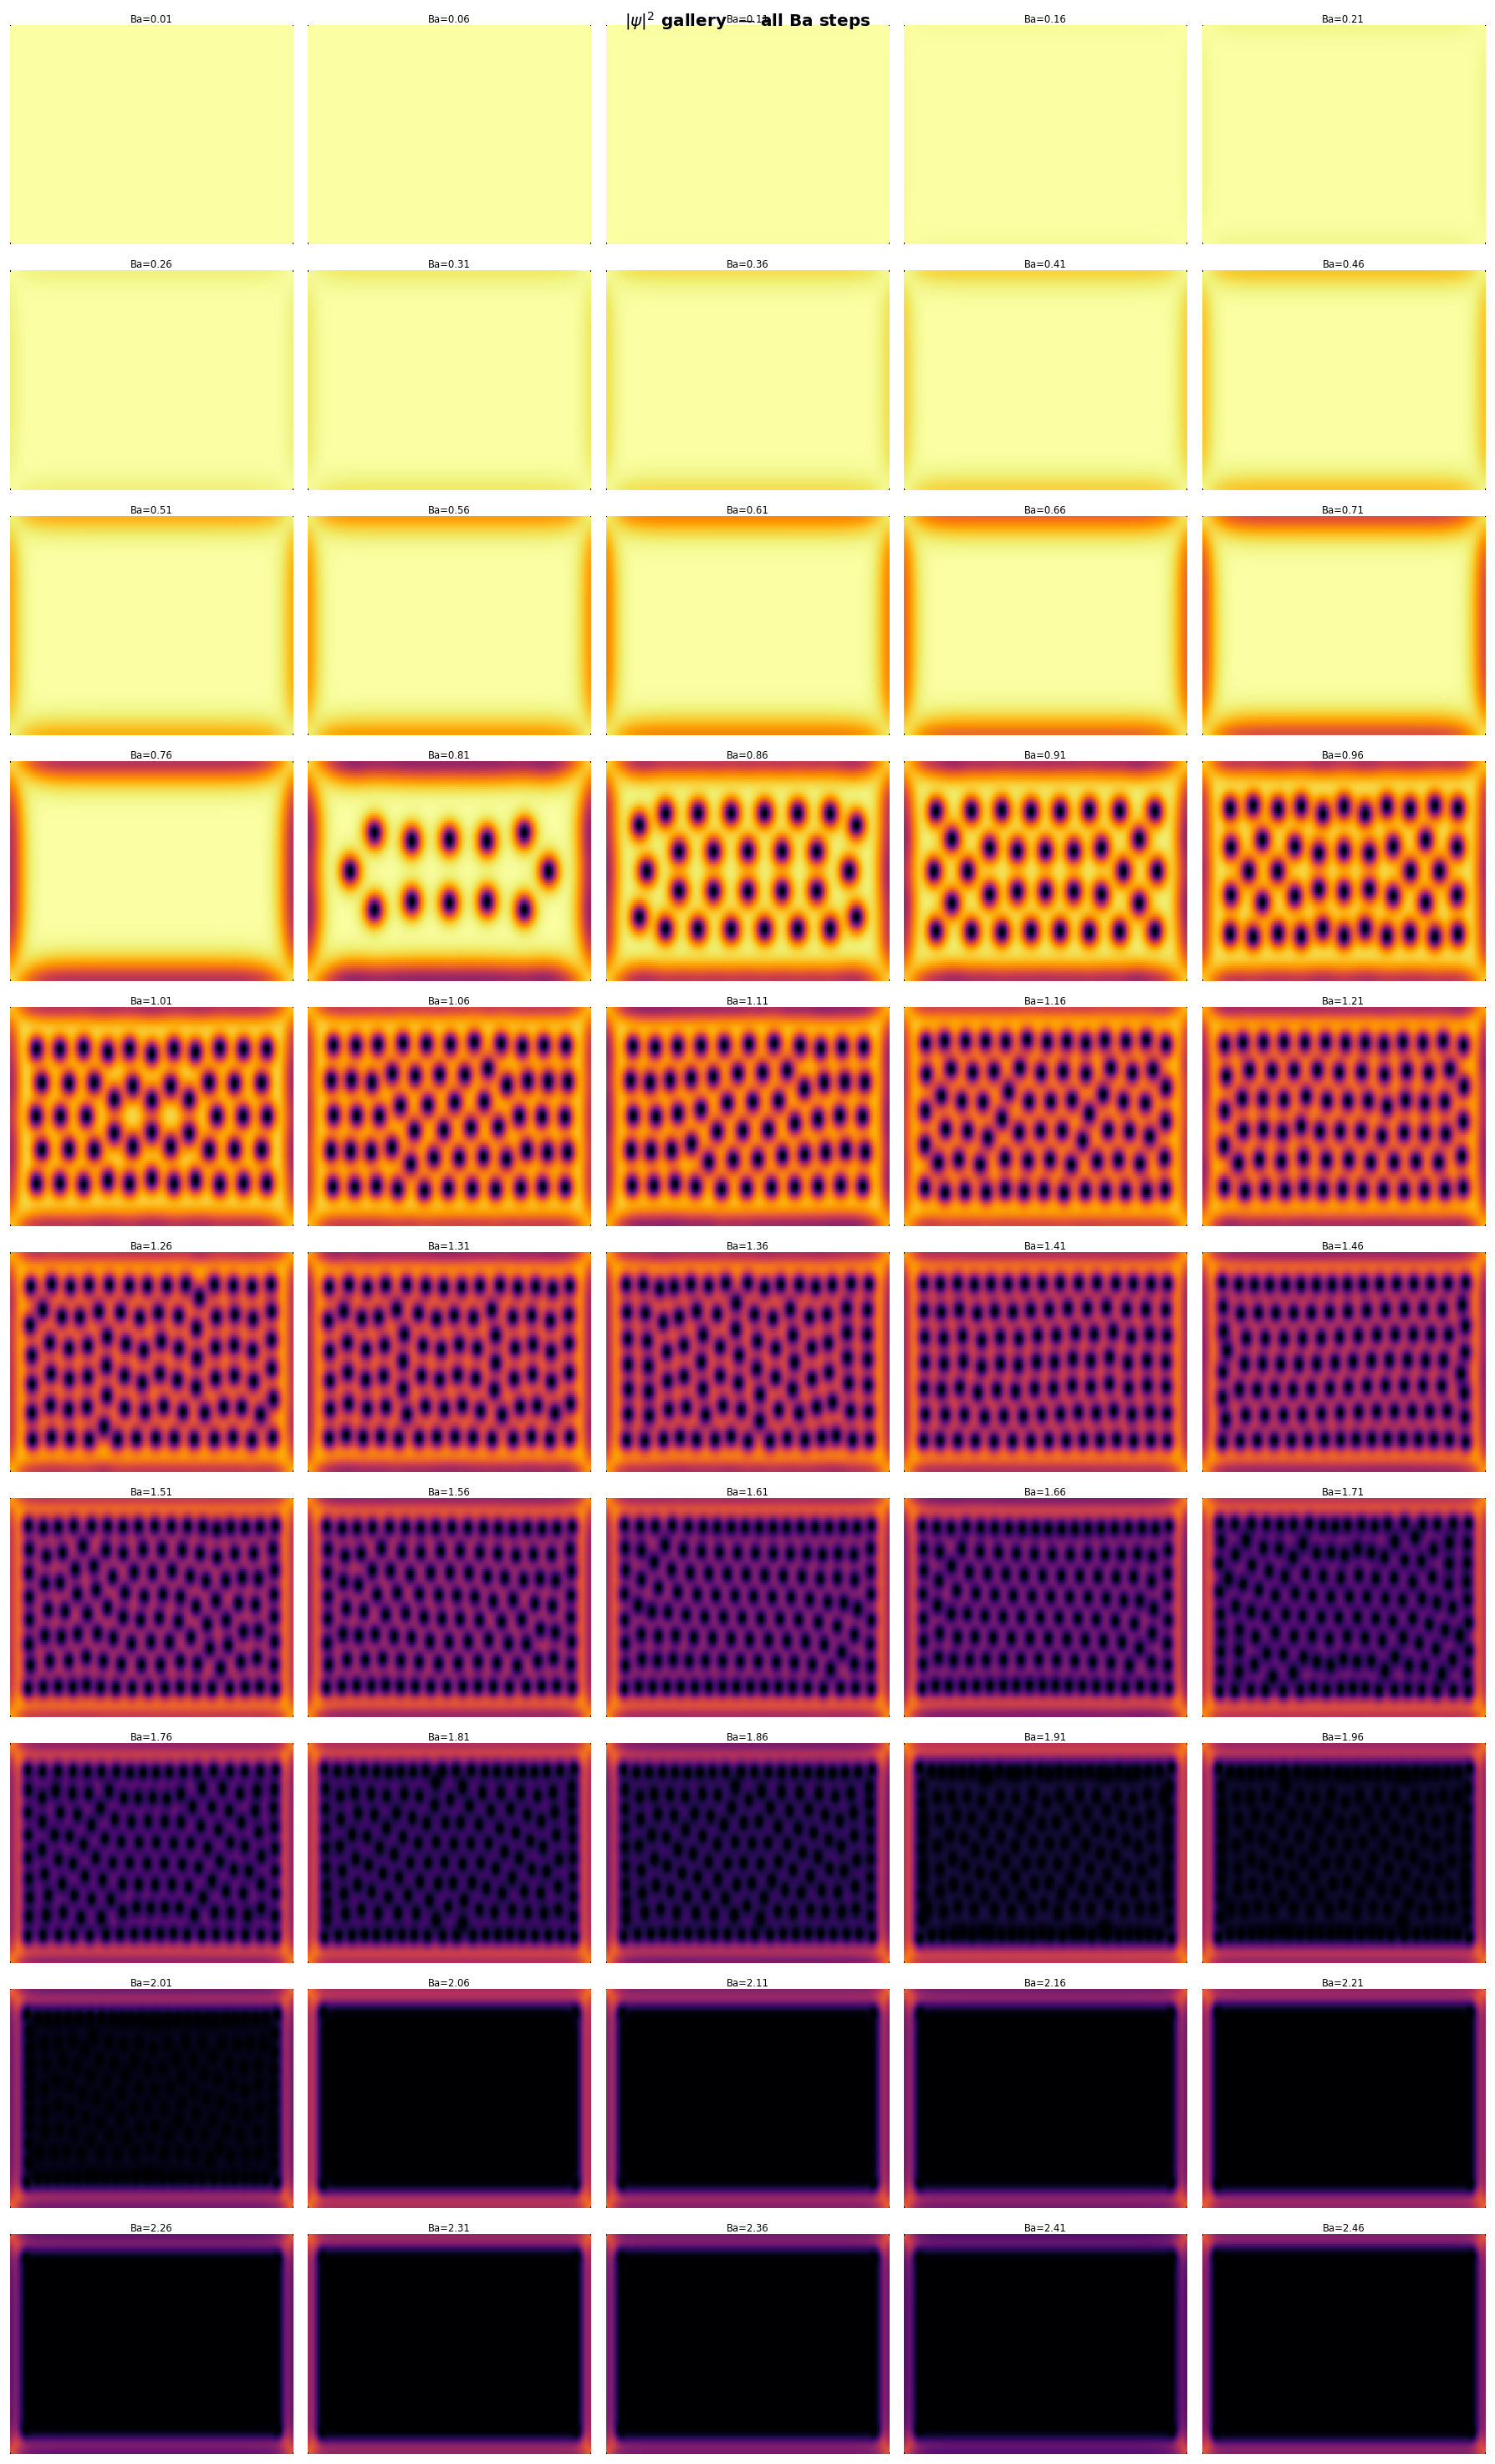
\includegraphics[width=\textwidth]{../figures/psi_gallery_zfc.png}
  \caption{Gallery of $|\psi|$ maps for all 50 field steps
           ($\Ba = 0.01$ to $2.46$, step $0.05$).
           The progressive vortex penetration and increasing core-overlap at
           high fields are visible across the panels.}
  \label{fig:psi_gallery}
\end{figure}

\begin{figure}[h!]
  \centering
  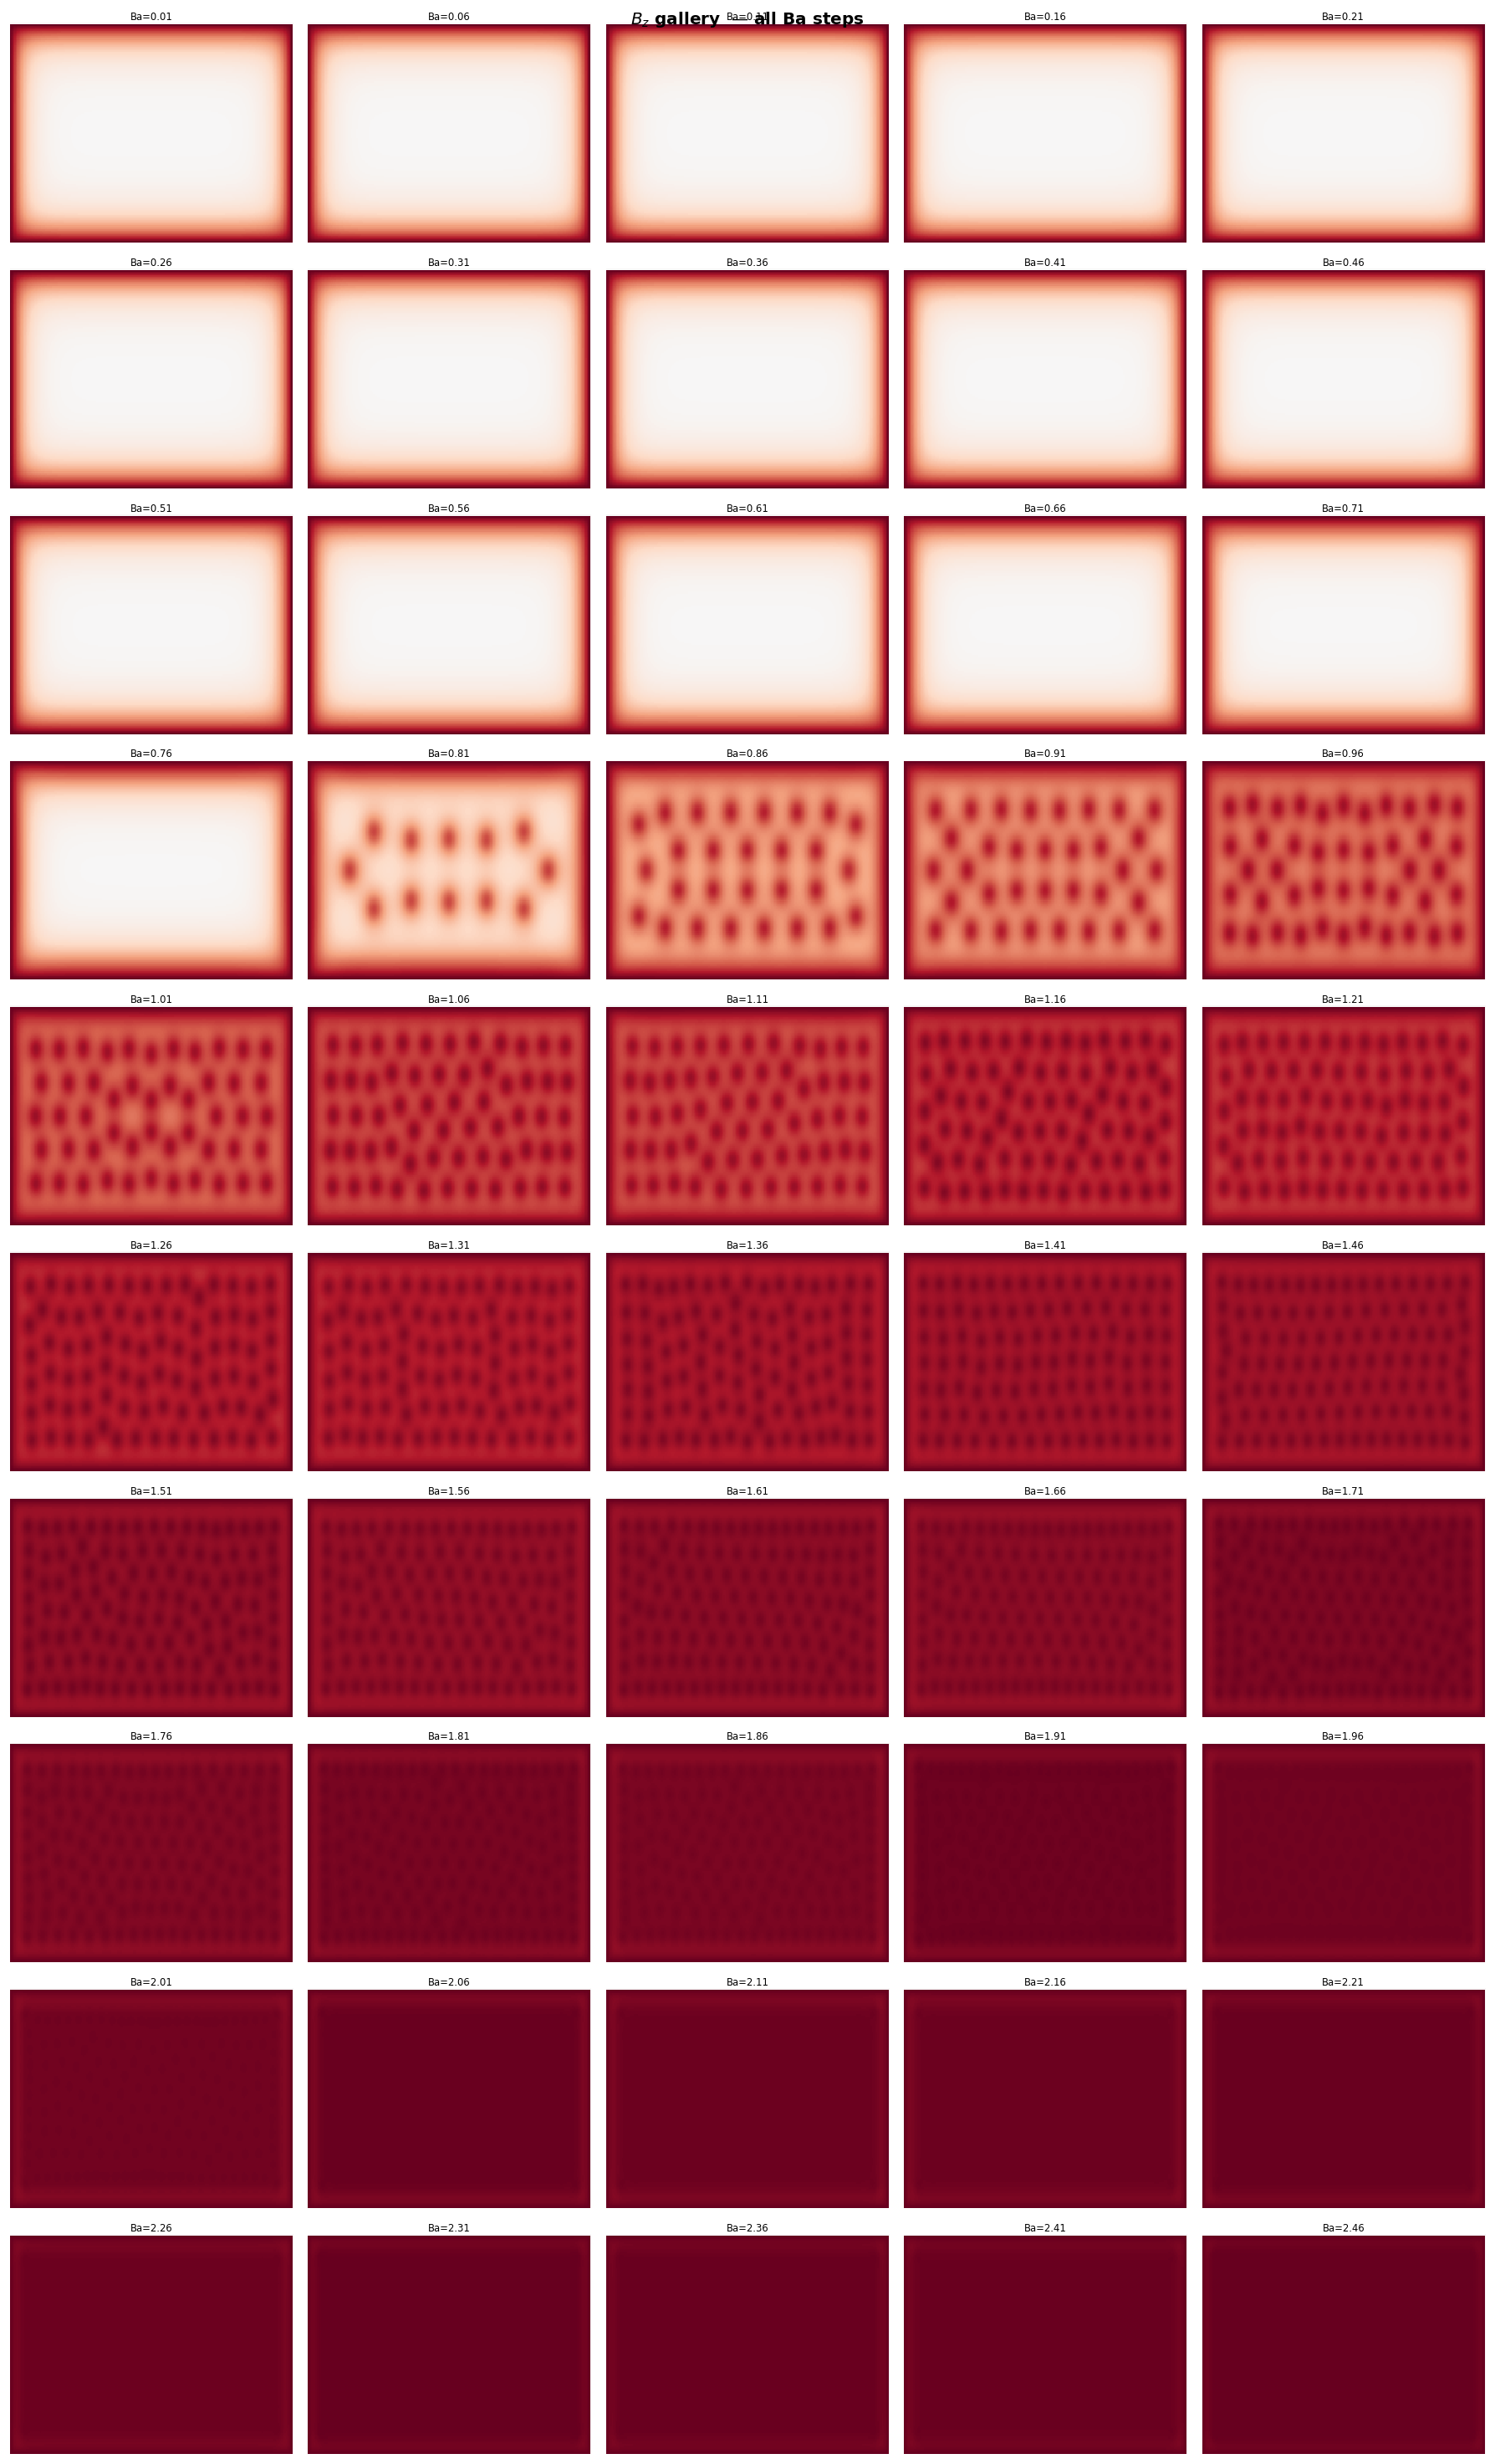
\includegraphics[width=\textwidth]{../figures/bz_gallery_zfc.png}
  \caption{Gallery of $B_z$ maps for all 50 field steps.
           Bright spots mark vortex cores where the local field is enhanced.}
  \label{fig:bz_gallery}
\end{figure}

Figures~\ref{fig:psi_gallery} and~\ref{fig:bz_gallery} show the complete
spatial evolution of the order parameter and field across all 50 field steps.
The onset of vortex penetration at $\Ba \approx 0.81$ and the gradual filling
of the sample are clearly visible.

\subsection{Supercurrent Distribution}

\begin{figure}[h!]
  \centering
  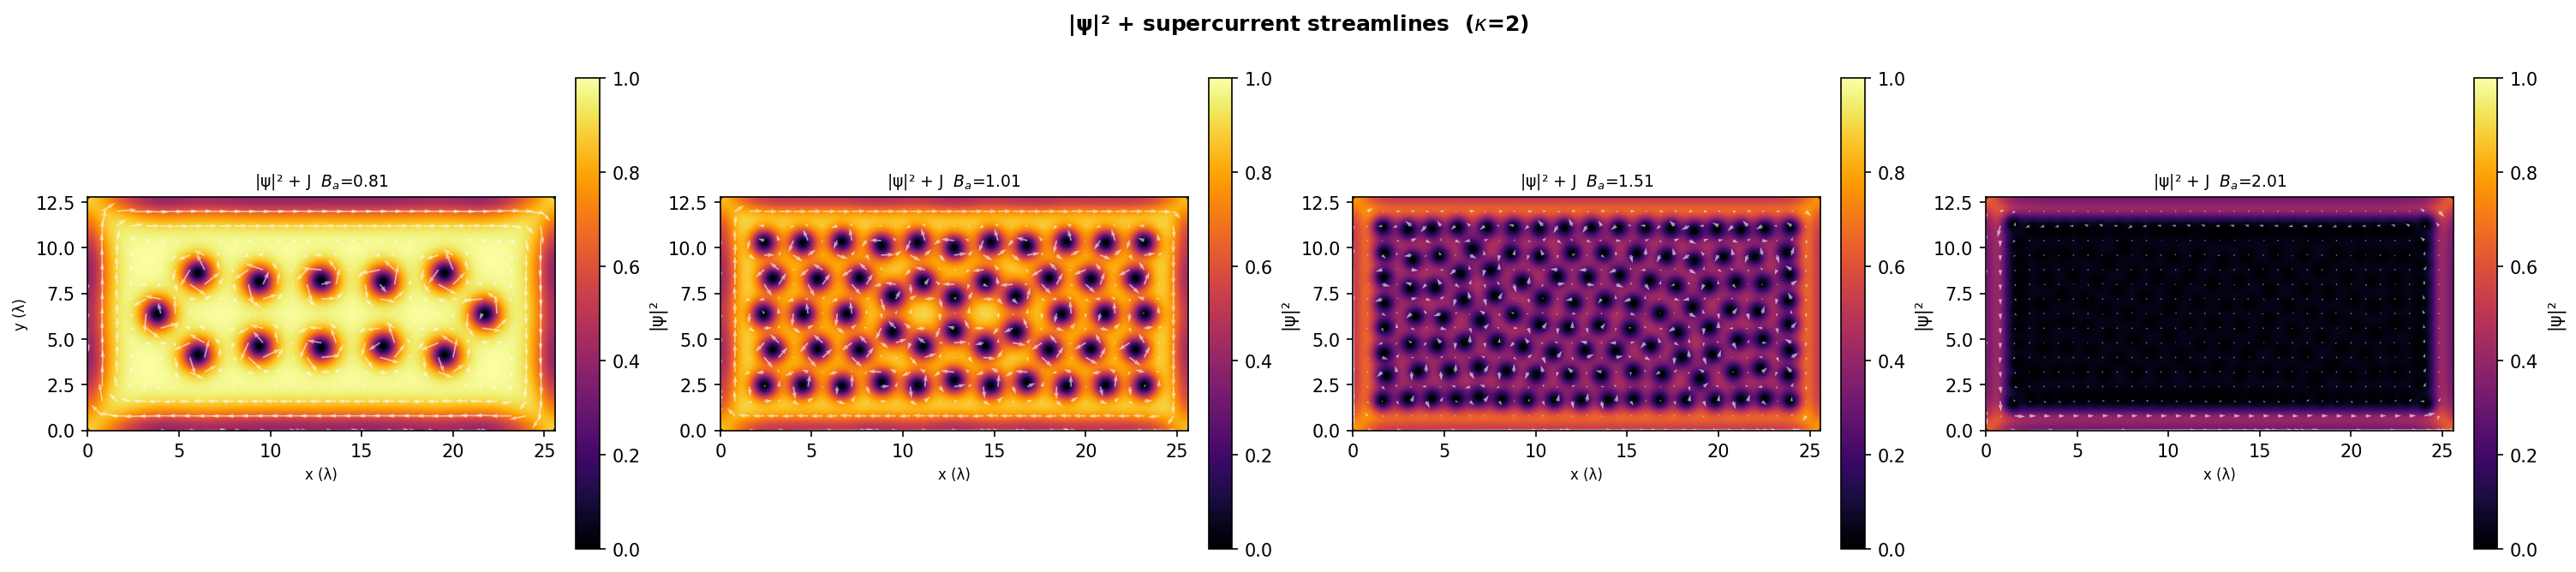
\includegraphics[width=\textwidth]{../figures/current_maps_zfc.png}
  \caption{Supercurrent density magnitude $|\Jvec_s|$ with streamlines
           overlaid on $|\psi|^2$, for four representative fields.
           Circular supercurrent loops around each vortex core are the
           microscopic origin of the diamagnetic response.}
  \label{fig:current}
\end{figure}

Figure~\ref{fig:current} shows the supercurrent density $\Jvec_s$, computed
from the gauge-invariant expression:
%
\begin{equation}
  \Jvec_s = \frac{1}{\kGL}\operatorname{Im}\!\left(\psi^*
  \left(\frac{1}{i}\nabla - \Avec\right)\!\psi\right).
  \label{eq:Js}
\end{equation}
%
Persistent circulating currents around each vortex core are clearly resolved.
At low fields, screening currents dominate near the sample boundary.

\subsection{Vortex Positions and Lattice Structure}

\begin{figure}[h!]
  \centering
  \begin{subfigure}[b]{0.48\textwidth}
    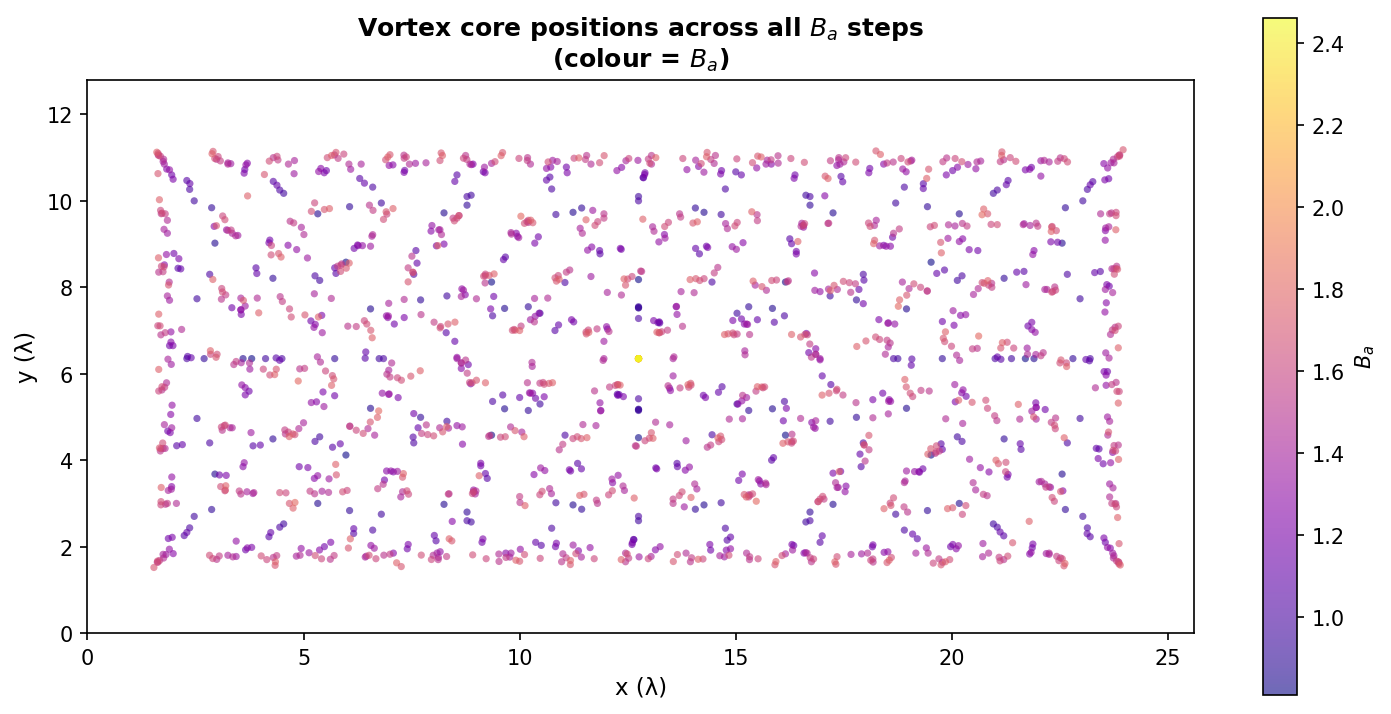
\includegraphics[width=\textwidth]{../figures/vortex_cores.png}
    \caption{Vortex core positions (colour = $\Ba$).}
    \label{fig:cores}
  \end{subfigure}\hfill
  \begin{subfigure}[b]{0.48\textwidth}
    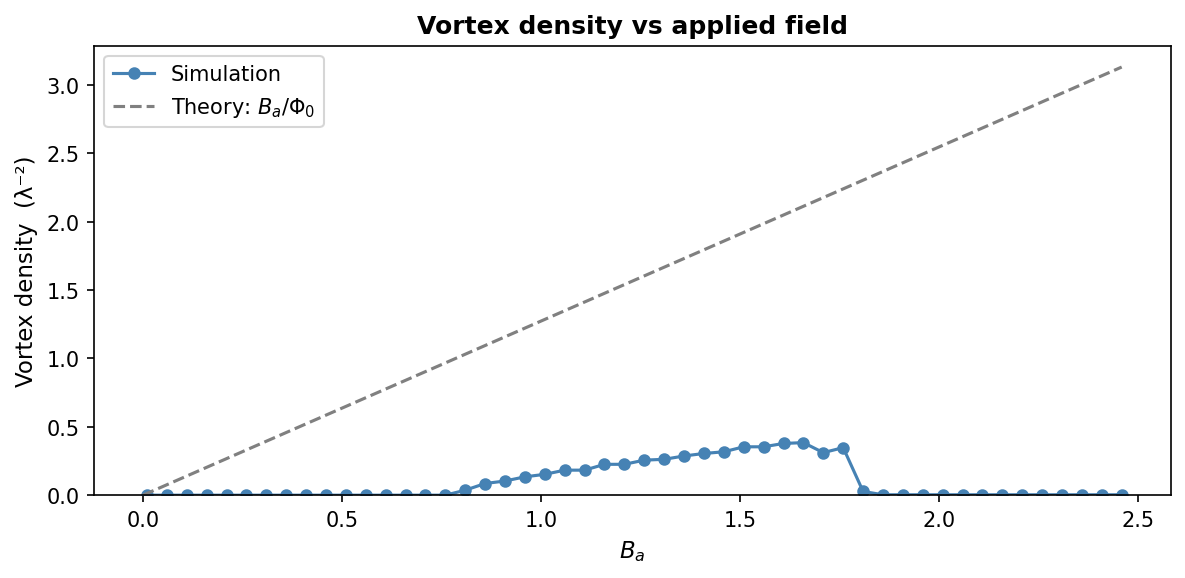
\includegraphics[width=\textwidth]{../figures/vortex_density.png}
    \caption{Vortex density vs applied field.}
    \label{fig:density}
  \end{subfigure}
  \caption{Vortex core analysis.}
  \label{fig:vortex}
\end{figure}

Figure~\ref{fig:cores} shows the accumulated vortex positions coloured by
field value.  The vortices nucleate from the sample edges and progressively
fill the interior.  Figure~\ref{fig:density} compares the measured areal
density $n_v = N_{\rm vor}/L_xL_y$ with the theoretical expectation
$n_v^{\rm th} = \Ba/\Phi_0$ for a fully penetrated sample.

\subsection{Hexatic Order Parameter}

\begin{figure}[h!]
  \centering
  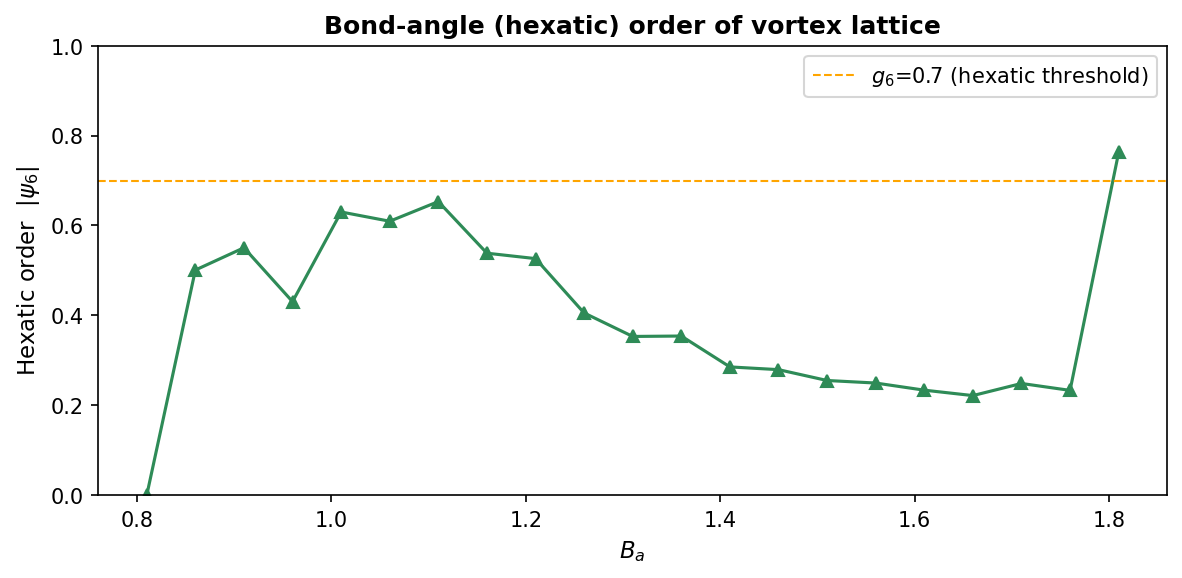
\includegraphics[width=0.65\textwidth]{../figures/lattice_order.png}
  \caption{Hexatic bond-order parameter $g_6$ vs applied field.
           $g_6 \to 1$ for a perfect triangular lattice; $g_6 \to 0$ for a
           disordered (liquid-like) vortex arrangement.}
  \label{fig:g6}
\end{figure}

The hexatic order parameter
%
\begin{equation}
  g_6 = \left|\frac{1}{N_{\rm vor}}\sum_{k=1}^{N_{\rm vor}}
        e^{6i\theta_k}\right|,
  \label{eq:g6}
\end{equation}
%
where $\theta_k$ is the average bond angle of the $k$-th vortex with its
neighbours, quantifies the degree of triangular (Abrikosov) lattice order.
Figure~\ref{fig:g6} shows that $g_6$ peaks at $\approx 0.63$ near
$\Ba \approx 1.01$--$1.11$, indicating a partially ordered vortex lattice.
The finite sample size and boundary effects limit the maximum attainable $g_6$.
At higher fields, increasing vortex density and core overlap suppress the order.

% ══════════════════════════════════════════════════════════════════════════════
\section{Discussion}
% ══════════════════════════════════════════════════════════════════════════════

The simulated $\Hcone \approx 0.81$ is consistent with the analytical
estimate for a GL superconductor with $\kGL = 2$:
%
\begin{equation}
  \Hcone \approx \frac{\ln\kGL}{\kGL\sqrt{2}}\,H_c
             \approx \frac{\ln 2}{2\sqrt{2}}\,H_c \approx 0.245\,H_c,
  \label{eq:hc1}
\end{equation}
%
where $H_c = 1/\sqrt{2}$ in the present dimensionless units ($H_c = \Phi_0/2\sqrt{2}\pi\xi\lam$).
This gives $\Hcone^{\rm th} \approx 0.173$, somewhat below the observed 0.81.
The discrepancy is expected: the Bean-Livingston surface barrier delays
vortex entry beyond the true $\Hcone$, and finite-size effects of the
$25.6\lam\times12.8\lam$ sample further raise the apparent threshold.

The peak vortex count $N_{\rm vor}^{\rm max} \approx 126$ at $\Ba = 1.66$
corresponds to an areal density $n_v \approx 1.66/\Phi_0$, in good agreement
with the expected value for a fully penetrated Abrikosov state.  The
subsequent decline in $N_{\rm vor}$ for $\Ba > 1.66$ reflects increasing core
overlap as the system approaches $\Hctwo$.

\paragraph{Note on the high-field vortex count.}
The winding-number estimator
$n_v = (2\pi)^{-1}\oint_{\partial\square}\nabla\theta\cdot d\mathbf{l}$
requires a well-defined phase $\theta = \arg\psi$.  At high applied fields
the vortex spacing $a_0 \propto \Ba^{-1/2}$ decreases below the coherence
length $\xi = 0.5\,\lam$, so adjacent cores overlap and their phase
singularities merge; the algorithm then counts a cluster of overlapping
cores as a single vortex.  Furthermore, as $|\psi|$ is globally suppressed
near $\Hctwo$, the phase becomes numerically noisy and the winding number
integral accumulates errors.

The \emph{true} number of flux quanta can be estimated from the mean local
field instead:
%
\begin{equation}
  N_v^{\rm true} = \frac{\langle B_z \rangle \cdot L_x L_y}{\Phi_0}
                 = \frac{(\Ba + M)\,L_x L_y}{\Phi_0},
  \label{eq:Nvtrue}
\end{equation}
%
where $\langle B_z\rangle = \Ba + M$ follows from the definition of the
magnetisation.  At $\Ba = 2.46$ this gives
$N_v^{\rm true} \approx 2.44 \times 25.6 \times 12.8 / (2\pi/\kappa^2)
\approx 127$, while the winding-number counter reports only 31 — a
fourfold undercount caused entirely by core overlap.  The magnetisation
remaining at $M \approx -0.016$ confirms that the sample is still
superconducting at this field, consistent with $\Hctwo > 2.46$.

\paragraph{Limitations.}
The simulation is two-dimensional ($z$-invariant) and does not capture
pancake-vortex physics in layered materials.  The sample is finite with
open boundaries; a larger sample would reduce boundary effects and allow
$g_6$ to approach unity in the well-ordered mixed state.  The upper critical
field $\Hctwo$ is not reached within the simulated range.

% ══════════════════════════════════════════════════════════════════════════════
\section{Conclusion}
% ══════════════════════════════════════════════════════════════════════════════

A GPU-accelerated TDGL simulation of a type-II superconductor ($\kGL = 2$)
on a $256\times128$ grid ($25.6\lam\times12.8\lam$) reproduces all key
features of the ZFC magnetisation curve:

\begin{itemize}
  \item Perfect Meissner diamagnetism for $\Ba < 0.76$.
  \item Discontinuous first-flux-entry at $\Ba^* \approx 0.81$ consistent
        with Bean-Livingston surface barrier nucleation.
  \item A well-defined Abrikosov mixed state with increasing vortex density
        and partial hexagonal lattice order ($g_6^{\rm max} \approx 0.63$).
  \item Core overlap and declining vortex count for $\Ba \gtrsim 1.66$,
        approaching but not reaching $\Hctwo$ within the simulated range.
\end{itemize}

These results validate both the gauge-invariant link-variable discretisation
and the Landau-gauge ZFC initialisation protocol implemented in the solver.

% ══════════════════════════════════════════════════════════════════════════════
\begin{thebibliography}{9}

\bibitem{gropp1996}
  W.~D. Gropp, H.~G. Kaper, G.~K. Leaf, D.~M. Levine, M.~Palumbo, and
  V.~M. Vinokur,
  \textit{Numerical simulation of vortex dynamics in type-II superconductors},
  J.\ Comput.\ Phys.\ \textbf{123}, 254 (1996).

\bibitem{abrikosov1957}
  A.~A. Abrikosov,
  \textit{On the magnetic properties of superconductors of the second group},
  Sov.\ Phys.\ JETP \textbf{5}, 1174 (1957).

\bibitem{bean1964}
  C.~P. Bean and J.~D. Livingston,
  \textit{Surface barrier in type-II superconductors},
  Phys.\ Rev.\ Lett.\ \textbf{12}, 14 (1964).

\bibitem{tinkham}
  M.~Tinkham,
  \textit{Introduction to Superconductivity}, 2nd ed.\
  Dover, New York (1996).

\end{thebibliography}

\end{document}
